\documentclass[twocolumn, 11pt]{article}%
\usepackage{amsmath, amssymb, esint}
\usepackage{graphicx, cuted, geometry, float, chemfig}

\geometry{
    a4paper,
    total={170mm,260mm},
}

\begin{document}

\begin{strip}
  \vspace*{\dimexpr-\stripsep}
  \begin{center}
      \Large\textbf{FISIKA 2}\\
      \large{Pertemuan 1 - Minggu 1 (772403)}\\
      \large{March 8, 2021}
   \end{center}
\end{strip}

\section{Hukum Coulomb}
        \paragraph{ } Hukum Coulomb membahas tentang gaya-gaya yang muncul dari interaksi antara 2 atau lebih partikel bermuatan. Gaya tarik timbul dari karena adanya 2 muatan yang berlawanan, sedangkan gaya tolak timbul karena adanya 2 benda yang muatannya sama (positif-positif, negatif-negatif). Hukum Coulomb dapat dirumuskan secara matematis menjadi
        \[F = k \frac{\mid q_1 q_2 \mid}{r^2} \]

        $k$ merupakan \textbf{konstanta elektrostatis} yang memiliki besar $8.988 \times 10^9\ Nm^2/C^2$ (atau sering dibulatkan dengan $8.988 \times 10^9\ Nm^2/C^2$). Nilai $k$ bisa dihitung dengan rumus $\displaystyle k=\frac{1}{4\pi \epsilon_0}$. Lalu $\epsilon_0$ adalah \textbf{Permitivitas Ruang Hampa} yang bernilai $8.85 \times 10^{-12}\ C^2/Nm^2$\\

        Rumus di atas tidak dapat menentukan arah dari gaya listrik (karena gaya merupakan besaran vektor yang punya nilai dan juga arah). Berikut adalah tabel informasi muatan dan juga massa partikel-partikel subatomik.

        \begin{table}[h!]
            \begin{center}
                \begin{tabular}{l|c|c}
                    \textbf{Particle} & \textbf{Charge} & \textbf{Mass}\\
                    \hline
                    Electron & $-1.6 \times 10^{-19}\ C$ & $9.11 \times 10^{-31}\ Kg$\\
                    Proton & $+1.6 \times 10^{-19}\ C$ & $1.673 \times 10^{-27}\ Kg$\\
                    Neutron & $0\ C$ & $1.675 \times 10^{-27}\ Kg$
                \end{tabular}
            \end{center}
        \end{table}

        \subsection{Gaya Listrik/Gaya Coulomb}
        Untuk mengetahui arah gayanya, digunakan rumus sebagai berikut
        \[\vec F_{12} = k \frac{q_1 q_2}{r^2} \hat r_{12} \]

        Perlu diketahui bahwa $\vec F_{12}$ adalah gaya pada muatan 1 oleh muatan 2. Sedangkan. $\vec F_{21}$ adalah gaya pada muatan 2 oleh muatan 1.
         
        \begin{center}
            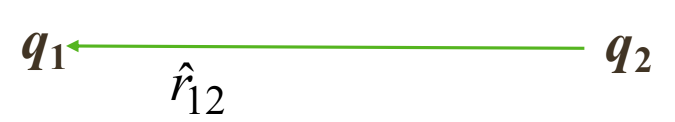
\includegraphics[width=150px]{1.png} 
        \end{center}

        $\hat r_{12}$ adalah vektor satuan dengan arah dari muatan 2 menuju muatan 1. Arah gaya bisa paralel atau anti-paralel terhadap vektor satuan ini, tergantung pada tanda relatif muatan.

        Lalu, rumus energi potensial listrik adalah
        \[E_p = k \frac{\mid q_1 q_2 \mid}{r} \]

        \subsection{Hukum III Newton pada Gaya Listrik/Gaya Coulomb}
        \begin{center}
           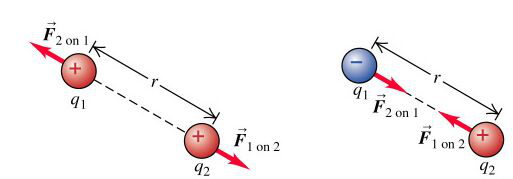
\includegraphics[width=200px]{2.png}
        \end{center}

        Pada saat objek-objek bermuatan saling berinteraksi (tarik-menarik ataupun tolak-menolak), maka gaya yang bekerja pada setiap objeknya \textbf{sama besar, tapi berlawanan arah.}
        \[\mid \vec F_{12}\mid\ =\ \mid \vec F_{21} \mid \]
       
\end{document}
